This section defines the reference frames used throughout this thesis. They are introduced to describe rigid body rotation and to define vectors in $\mathbb{R}^3$. A reference frame is a term used to describe a right-handed three-dimensional Cartesian coordinate system that is described by three mutually perpendicular unit vectors. Calculations are made easier by using multiple reference frames that have been carefully placed. They are introduced in figure \ref{fig:three graphs}. They are divided into two Geo-based frames and two satellite based frames.

\section{Earth-Based Reference Frames}
\subsection{Earth Centered Earth Fixed Frame}
The origin of ECEF system is the earth's center. This frame of reference rotates with the earth which means if there’s any fixed point on the surface of the earth, its coordinates will not change. The $x^e$axis is passing through the Equator and Greenwich Meridian intersection. The $z^e$ axis is passing by the North Pole. The $y^e$ axis is orthogonal to $x^e$ axis and $z_e$ axis. The configuration is shown in figure \ref{fig:ECEF}.

\subsection{Earth Centered Inertial Frame}
ECI coordinate system is a reference system where the origin is at the earth's center of mass. Unlike the ECEF frame the ECI frame doesn't rotate with the earth. The $x^i$ axis is fixed towards the mean vernal equinox. The $z^i$ axis corresponds to the mean north celestial pole of epoch J2000.  The $y^i$ axis is the vector product of the $z^i$ and $x^i$ axes. The configuration is shown in figure \ref{fig:ECI}

\begin{figure}[H]
     \centering
     \begin{subfigure}[b]{0.4\textwidth}
         \centering
         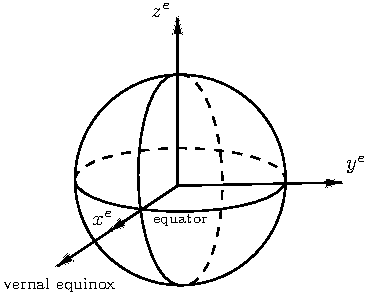
\includegraphics[width=\textwidth]{Figures/ECI.pdf}
         \caption{Earth centered inertial reference frame}
         \label{fig:ECI}
     \end{subfigure}
     \hfill
     \begin{subfigure}[b]{0.4\textwidth}
         \centering
         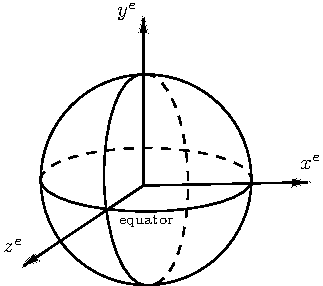
\includegraphics[width=\textwidth]{Figures/ECEF.pdf}
         \caption{Earth centered Earth fixed reference frame}
         \label{fig:ECEF}
     \end{subfigure}
     \hfill
     \begin{subfigure}[b]{\textwidth}
         \centering
        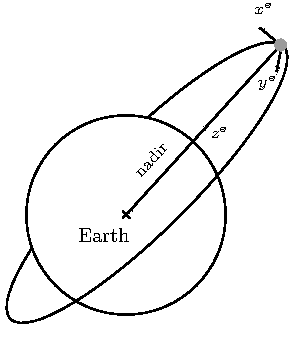
\includegraphics[width=0.5\textwidth]{Figures/ORF.pdf}
         \caption{Orbit reference frame}
         \label{fig:ORF}
     \end{subfigure}
     \hfill
     \begin{subfigure}[b]{0.4\textwidth}
         \centering
        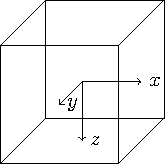
\includegraphics[width=0.5\textwidth]{Figures/BRF.pdf}
         \caption{Satellite body reference frame}
         \label{fig:SBF}
     \end{subfigure}
        \caption{The reference frames used in this thesis.}
        \label{fig:three graphs}
\end{figure}  %% Coordinate Systems Diagram

\begin{comment}
\subsection{The Geodetic Coordinate System}
The geodetic coordinate system; also called the Latitude and Longitude coordinate system. It consists of the geodetic grid for the planet which is mainly parallel East/West lines representing the latitude and North/South lines representing the longitude which intersect at the poles. The lines of the Latitude and Longitude are ordered by the angle they subtend relative to a certain reference. 

The latitude angle $\phi$ is the angle between the plane of the equator and the point of interest. The zero reference for the latitude is the Equator. The longitude geodetic location does not have an intuitive understanding of distance because the longitude lines are not parallel. The zero reference is the Greenwich Meridian.
\end{comment}



\section{Satellite-Based Reference Frames}
\subsection{Orbit reference frame}
The ORF maintains its orientation with respect to the Earth and tracks the satellite in its orbit. The attitude of the satellite with respect to this coordinate system is also referred to as roll, pitch, and yaw. The $z^o$ axis points out from the satellite along the geocentric radius vector. The $y^o$ axis is normal to the orbital plane which is created from the position vector and velocity vector. The $x^o$ axis is normal to the position vector and positive in the direction of the velocity vector.it is also aligned with the velocity vector only for circular orbits. The configuration is shown in figure \ref{fig:ORF}.

\subsection{Satellite body reference frame}
This coordinate system is used to define ADCS measurements. The origin of this system is the center of mass. The axis are chosen as the $x^b$ points through the front of the satellite. The $y^b$ points to the right of the $x^b$ and is perpendicular to it. The $z^b$ is pointing down the satellite and perpendicular to the $x^b - y^b $ plane.

%\section{Coordinates Transformation}



\clearpage